\documentclass[11pt, oneside]{article}
\usepackage{geometry}
\geometry{letterpaper}
\usepackage{setspace} 
\usepackage{lineno} 
%
\usepackage[parfill]{parskip}
\usepackage{amssymb}
\usepackage{amsmath}
\usepackage{dsfont}
\usepackage{mathptmx} 
%
\usepackage{graphicx}
\usepackage[labelfont=bf]{caption} 
\usepackage{float} 
%
\usepackage[
	style=authoryear,
	citestyle=authoryear,
	maxbibnames=6,
	giveninits=true,
	backend=bibtex,
	url=false,
	doi=false,
	isbn=false,
	eprint=false
	]{biblatex}
\addbibresource{references.bib}
\AtEveryBibitem{\clearfield{note}}
%
%% add S in front of figure and table names
\newcommand{\beginsupplement}{%
        \setcounter{table}{0}
        \renewcommand{\thetable}{S\arabic{table}}%
        \setcounter{figure}{0}
        \renewcommand{\thefigure}{S\arabic{figure}}%
     }

\title{Supplementary information file for \textit{Fast fitting of neural ordinary differential equations by Bayesian neural gradient matching to infer ecological interactions from time series data}}
\author{Willem Bonnaff\'e$^{1,2}$ \& Tim Coulson$^2$}
\date{}

\begin{document}
\maketitle
\pagenumbering{gobble}

1. Big Data Institute, University of Oxford, Old Road Campus, Oxford OX3 7LF 

2. Department of Biology, University of Oxford, Zoology Research and Administration Building, 11a Mansfield Road, Oxford OX1 3SZ 

\textbf{Contact:}
Willem Bonnaff\'e, 128 Southfield Park, Oxford, OX4 2BA, UK (w.bonnaffe@gmail.com)

\textbf{Statement of authorship:}
Willem Bonnaff\'e designed the method, performed the analysis, wrote the manuscript; 
Tim Coulson led investigations, provided input for the manuscript, commented on the manuscript.

% \newpage
\tableofcontents

\newpage
% \section{Supplementary}
\appendix
\beginsupplement
\pagenumbering{arabic}

\section{Bayesian regularisation}

The fitting of the models is performed in a Bayesian framework, considering normal error structure for the residuals, and normal prior density distributions on the parameters,

\vspace{-0.5cm}
\begin{equation}
	p(\omega | \mathcal{D}) \propto  p(\mathcal{D} | \omega) p(\omega),
\end{equation}

where $\theta$ is the parameter vector of the model, and $\mathcal{D}$ the evidence, namely the data that the model is fitted to.
Assuming a normal likelihood for the residuals given the evidence we get

\vspace{-0.5cm}
\begin{equation}
	p( \mathcal{D} | \omega) = \prod_{i=1}^{N} \frac{1}{\sqrt{2\pi\sigma^2}}  \exp \left\{ -\frac{e_i(\mathcal{D},\omega)^2}{2\sigma^2}  \right\},
\end{equation}

where $e_i(\mathcal{D},\omega)$ are the residuals of the model given the parameters, and the evidence. 
In the case of the interpolation, the residuals correspond to the observation error $\epsilon^{(o)}$ (Eq. 3).
In the case of the NODE approximation, they correspond to the process error $\epsilon^{(p)}$ (Eq. 7).
$N$ is the number of data points, either observations in the case of the interpolation, $N^{(o)}$, or interpolated points in the case of the NODE fitting, $N^{(p)}$.

The prior probability density functions for the parameters are given by

\vspace{-0.5cm}
\begin{equation}
	p(\omega) = \prod_{j=1}^{M} \frac{1}{\sqrt{2\pi\delta_j^2}}  \exp \left\{ -\frac{\omega_j^2}{2\delta_j^2}  \right\},
\end{equation}

where $M$ is the number of parameters in the models.
The parameter $\delta_j$ controls the dispersion of the priors, and thereby the complexity/level of constraint of the model.

Bayesian regularisation consists in constraining the values of the parameters in the model to be close to a desired value. 
Usually, parameters are constrained by choosing normal priors centered about 0.
In this case, the standard deviation of the normal priors, $\delta$, governs the range of values that the parameters can take, and hence constrains more or less strongly the behaviour of the model (\cite{Cawley2007}).
% There is no standard approach for choosing $\delta$.
Low values of dispersion may increase constraint on parameters too drastically, which would lead to underfitting, and result in a reduction of the variance of parameter estimates and bias mean estimates towards 0.
In contrast, too high values of dispersion may lead to overfitting, by allowing for more complex shapes.
To account for this, we optimise models on the second-level of inference.
This means that we are finding the optimal value of $\delta$, in addition to optimising the model parameters. 
% Performing inference on the second level means that we are trying to find the appropriate value of the dispersion of the priors, in other words, the appropriate level of constraint on the model. 

In practice, choosing the level of constraint is difficult, Cawley and Talbot hence developed a criterion to perform model selection on the second level of inference.
They proposed to optimise the marginal posterior distribution by averaging out the dispersion of the priors.
With an improper Jeffrey's hyperprior, $p(\xi) \propto \frac{1}{\xi}$, on the dispersion parameters, the dispersion can be integrated out, leaving us with a formula for the posterior that only depends on the parameters of the model,

\vspace{-0.5cm}
\begin{equation}
	\log P(\omega | \mathcal{D}) \propto - \frac{N}{2} \log \left(\sum_{i=1}^{N} e_i(\mathcal{D},\omega)^2\right) - \frac{M}{2} \log \left(\sum_{j=1}^{M} \omega_{j}^2 \right),
\end{equation}

where $P(\omega|\mathcal{D})$ denotes the marginal posterior density, $\mathcal{D}$ denotes the evidence, $N$ and $M$ denote the number of data points and parameters, respectively, $e_i$ denote the residuals, and $\omega$ denote the parameters of the model.
The construction is elegant because it is not sensitive to the choice of prior hyperparameters, and simple as it amounts to optimising the log of the sum of squares, rather than the sum of squares (in the case of normal ordinary least square).

One of the drawbacks of this construction is that the marginal posterior density is not finite when the parameters are 0, which can lead to underfitting.
In this paper we use a modified criterion, which corrects for that problem,

\vspace{-0.5cm}
\begin{equation}
	\log P(\omega | \mathcal{D}) \propto - \frac{N}{2} \log \left(1 + \sum_{i=1}^{N} e_i(\mathcal{D},\omega)^2\right) - \frac{M}{2} \log \left(1 + \sum_{j=1}^{M} \omega_{j}^2 \right),
\end{equation}

where the marginal posterior density depends only on the residuals of the model when the parameters are equal to 0, and otherwise depends on both the parameters and the residuals. 
This construction can be obtained by adding an exponential correction to the improper Jeffrey's hyperprior that Cawley and Talbot used in their original study, namely $p(\xi) \propto \frac{1}{\xi} \exp\left\{- \xi/2 \right\}$, where $\xi$ is the regularisation parameter. 

We provide below details of the calculation of this modified criterion, starting by averaging out the regularisation parameter.
We let $\xi := 1/\delta^2$, assuming that all parameters are controlled by the same regularisation parameter, which gives the following equation for the prior distribution,

\vspace{-0.5cm}
\begin{equation}
    p(\omega | \xi) = \prod_{j=1}^{M} \frac{1}{\sqrt{2\pi/\xi}}  \exp \left\{ -\frac{\xi}{2} \omega_j^2 \right\}.
\end{equation}

To follow the proof given by Cawley and Talbot we further use the following notation, $d := M$, $Z_\Omega := \left( 2\pi / \xi \right)^{d/2}$, and $\Omega := \sum_j \omega_j^2$, which yields

\vspace{-0.5cm}
\begin{equation}
    p(\omega | \xi) = {Z_\Omega(\xi)}^{-1}  \exp \left\{ -\frac{\xi}{2} \Omega(\omega)\right\}.
\end{equation}

We can then integrate out the regularisation parameter by computing the marginal prior distribution,

\vspace{-0.5cm}
\begin{equation}
    P(\omega) = \int p(\omega | \xi) p(\xi) d\xi.
\end{equation}

This expression can be solved analytically with the right choice of prior. 
Cawley and Talbot use $p(\xi) \propto 1/\xi$, but instead we choose $p(\xi) \propto 1/\xi \exp\{-\xi/2\}$.
By assuming positive support for $\xi$ and expanding out the marginal prior distribution we get,

\vspace{-0.5cm}
\begin{equation}
\begin{aligned}
    P(\omega) &= \int_0^{\infty} \left( \frac{2\pi}{\xi} \right)^{-d/2}  \exp \left\{ -\frac{\xi}{2} \Omega(\omega)\right\} \frac{1}{\xi} \exp\left\{-\frac{\xi}{2}\right\} d\xi\\
    &= (2\pi)^{-d/2} \int_0^{\infty} \xi^{d/2-1} \exp \left\{ -\frac{\xi}{2} \left(\Omega(\omega) + 1 \right) \right\} d\xi \\
\end{aligned}
\end{equation}

We use the gamma integral, $\int_{0}^{\infty} x^{v-1} \exp\{-\mu x\} = \Gamma(v)/\mu^{v}$ (\cite{Cawley2007}), to obtain,

\vspace{-0.5cm}
\begin{equation}
    P(\omega) = (2\pi)^{-d/2} \frac{\Gamma(d/2)}{(1/2)^{d/2}\left(\Omega(\omega)+1\right)^{d/2}} 
\end{equation}

Finally, by applying the logarithm and discarding constants, we obtain the final expression for the marginal prior distribution,

\vspace{-0.5cm}
\begin{equation}
\begin{aligned}
    \log P(\omega) &\propto - \frac{d}{2} \log \left(\Omega(\omega)+1\right) \\
    &\propto -\frac{M}{2} \log \left(1 + \sum_j^M \omega_j^2 \right)
\end{aligned}
\end{equation}

The same procedure can be applied to derive the marginal likelihood, by noting $d := N$, $\xi := 1/\sigma^2$, $Z_\Omega := (2\pi/\xi)^{d/2}$, $\Omega(\omega) := \sum_i e_i^2$.

%%
\newpage
\section{Complementary results benchmark analysis}

%% figure
% \newpage
\begin{figure}[H]
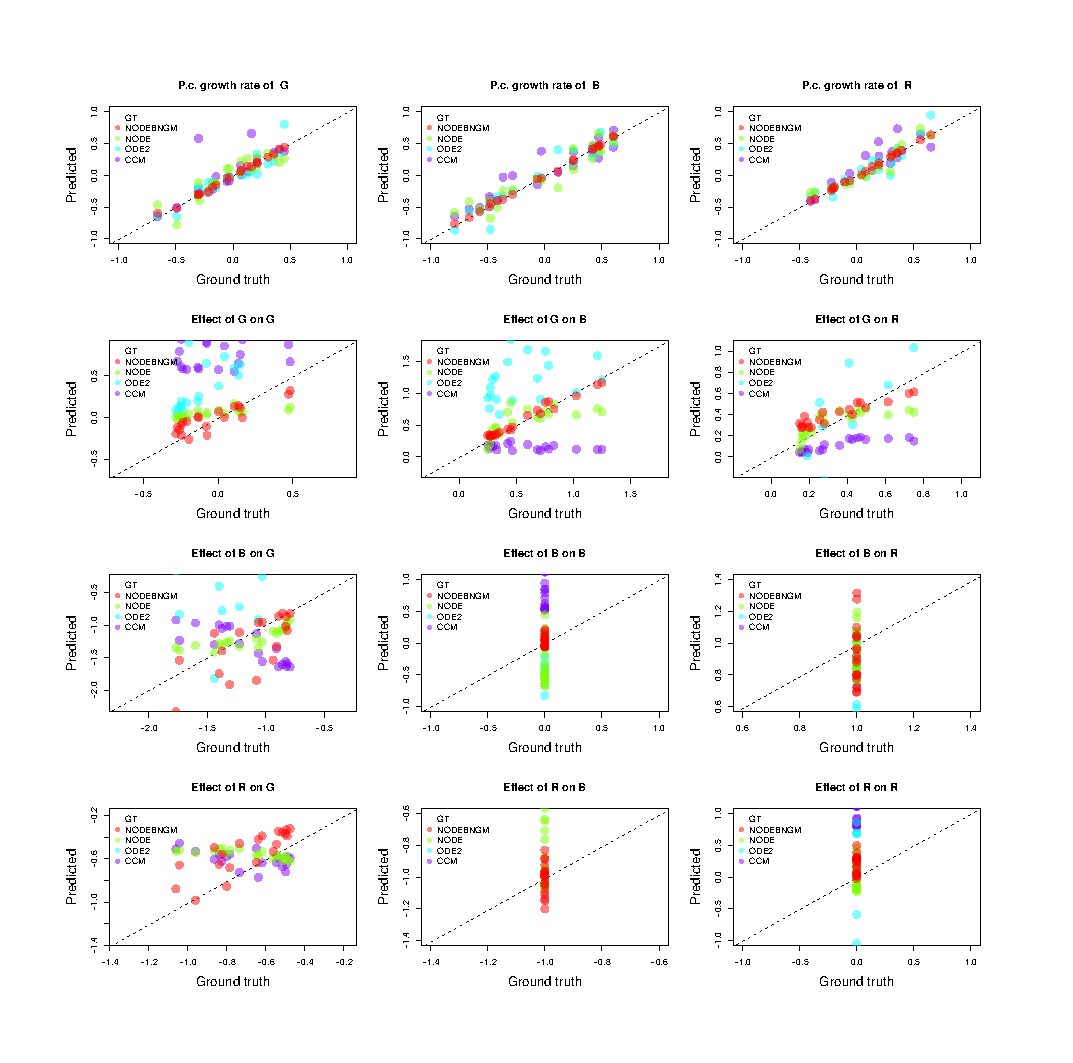
\includegraphics[width=1\linewidth,page=1]{figures/figures_supplementary.pdf}
\caption{
    \textbf{Train set accuracy of predicted per-capita growth rates and effects estimated by NODEBNGM, standard NODEs, ODE2, and CCM.}
    The NODEBNGM method (nonparametric) involves fitting a NODE system by Bayesian neural gradient matching (BNGM). 
    The NODE method (nonparametric) involves fitting a NODE system with an ODE solver. 
    The ODE2 method (parametric) involves fitting an ODE system with polynomial functions of species densities with an ODE solver. 
    The CCM method (nonparametric) involves computing locally linear approximations of the state space. 
    For each method, we trained 30 models on the two first thirds of the artificial time series where ground truth is known (Fig. 2). 
    For each plot, the x-axis corresponds to the ground truth, known from the equations that generated the artificial time series, and the y-axis corresponds to the prediction of the best model. 
    Effects are computed as the sensitivity (i.e. derivative) of the per-capita growth rate with respect to each species density G, B, and R, namely the prey, intermediate and top predator.
}
\end{figure}
\newpage

%% figure
% \newpage
\begin{figure}[H]
\includegraphics[width=1\linewidth,page=2]{figures/figures_supplementary.pdf}
\caption{
    \textbf{Test set accuracy of predicted per-capita growth rates and effects estimated by NODEBNGM, standard NODEs, ODE2, and CCM.}
    The NODEBNGM method (nonparametric) involves fitting a NODE system by Bayesian neural gradient matching (BNGM). 
    The NODE method (nonparametric) involves fitting a NODE system with an ODE solver. 
    The ODE2 method (parametric) involves fitting an ODE system with polynomial functions of species densities with an ODE solver. 
    The CCM method (nonparametric) involves computing locally linear approximations of the state space. 
    For each method, we trained 30 models on the two first thirds of the artificial time series where ground truth is known (Fig. 2). 
    For each plot, the x-axis corresponds to the ground truth, known from the equations that generated the artificial time series, and the y-axis corresponds to the prediction of the best model. 
    Effects are computed as the sensitivity (i.e. derivative) of the per-capita growth rate with respect to each species density G, B, and R, namely the prey, intermediate and top predator.
}
\end{figure}
\newpage

%% figure
% \newpage
\begin{figure}[H]
\includegraphics[width=1\linewidth,page=3]{figures/figures_supplementary.pdf}
\caption{
    \textbf{Effects and contributions inferred by standard NODEs.}
    The standard NODE model nonparametrically approximates the per-capita growth rate of the 3 species with an ANN featuring a single layer, 3 input nodes, 10 hidden nodes, 3 outputs.
    30 models are fitted to the two first third of the time series using BFGS and a Runge-Kutta ODE solver.
    The graphs present the predictions obtained for the model that maximises posterior density of the network parameters given the time series.
    We estimate the direction of ecological interactions (effects) by computing the derivative of the per-capita growth rate approximations with respect to each density.
    Finally, we compute the strength of ecological interactions (contributions) by multiplying the interpolated dynamics of each population with its effects.
}
\end{figure}
\newpage

%% figure
% \newpage
\begin{figure}[H]
\includegraphics[width=1\linewidth,page=4]{figures/figures_supplementary.pdf}
\caption{
    \textbf{Effects and contributions inferred by parametric ODE.}
    The ODE2 model parametrically approximates the per-capita growth rate of the 3 species with second order polynomial functions.
    30 models are fitted to the two first third of the time series using BFGS and a Runge-Kutta ODE solver.
    The graphs present the predictions obtained for the model that maximises posterior density of the network parameters given the time series.
    We estimate the direction of ecological interactions (effects) by computing the derivative of the per-capita growth rate approximations with respect to each density.
    Finally, we compute the strength of ecological interactions (contributions) by multiplying the interpolated dynamics of each population with its effects.
}
\end{figure}
\newpage

%% figure
% \newpage
\begin{figure}[H]
\includegraphics[width=1\linewidth,page=5]{figures/figures_supplementary.pdf}
\caption{
    \textbf{Effects and contributions inferred by CCM.}
    The CCM method nonparametrically approximates the state space from which it derives the sensitivity of population dynamics to a change in the density of the each species.
    We use the rEDM implementation and derived our code from the three species example provided in the package tutorial (v1.13.1, \cite{Sugihara2012}).
    We calculated the dynamics and per capita growth rate using finite differences, as the standard library does not readily provide estimates.
    The effects correspond to the s-map coefficients.
    Finally, we compute the strength of ecological interactions (contributions) by multiplying the interpolated dynamics of each population with its effects.
}
\end{figure}
\newpage


%%
\newpage
\section{Complementary results case study 2 replicate A}

%% figure
% \newpage
\begin{figure}[H]
\includegraphics[width=1\linewidth,page=6]{figures/figures_supplementary.pdf}
\caption{
    \textbf{Interpolation of state and dynamics of algae, flagellate, and rotifer density in replicate A.}
    Graph a., c., and e. display the neural interpolation of the population density of algae (G), flagellate (B), and rotifer (R), respectively (obtained with Eq. 7). 
    Graph b., d., and f. show the corresponding interpolated dynamics, obtained by differentiating the interpolation of the states with respect to time (Eq. 5).
    The shaded areas represent the 90\% confidence interval on estimates, obtained by anchored ensembling of the log marginal posterior distribution (Eq. 7) (\cite{Pearce2018}).
    Time series are obtained from digitising the time series in \cite{Hiltunen2013}.
}
\end{figure}
\newpage

%% figure
\newpage
\begin{figure}[H]
\includegraphics[width=1\linewidth,page=7]{figures/figures_supplementary.pdf}
\caption{
    \textbf{Cross-validation plot of the NODE analysis of replicate A.}
    The x-axis of the graphs correspond to the standard deviation of the prior distribution of the NODE parameters, which constrains the nonlinearity of the nonparametric approximation of the NODEs.
    Small values of standard deviation correspond to a linear model, while higher values (towards 0.5) correspond to a highly nonlinear model.
    Time series are split in three thirds to create a train, validation, and test set. 
    The model is fitted to the train set for increasing value of standard deviation (from 0.05 to 0.5 by 0.05 increments), and evaluated on the validation set.
    Graph a., c., and e. show the log likelihood of the NODE system fitted by BNGM to the train set of algae, flagellate, and rotifer, respectively.
    Graph b., d., and f. show the log likelihood of the fitted NODE, evaluated on the corresponding validation set.
    The shaded areas represent the 90\% confidence interval on estimates, obtained by anchored ensembling of the log posterior distribution (Eq. 8) (\cite{Pearce2018}).
}
\end{figure}
\newpage

%% figure
\newpage
\begin{figure}[H]
\includegraphics[width=1\linewidth,page=8]{figures/figures_supplementary.pdf}
\caption{
    \textbf{Drivers of dynamics of algae, flagellate, and rotifer in replicate A.}
    This figure displays the NODE nonparametric approximations of the per-capita growth rate of algae (a., b., c.), flagellate (d., e., f.), and rotifer (g., h., i.).
    We obtain the NODE approximations (a., d., g., solid line) by fitting the interpolated per-capita growth rates (black dots) with ANNs that take population densities as input.
    We then estimate the direction of ecological interactions (effects, b., e., h.) by computing the derivative of the NODE approximations with respect to each density.
    Finally, we compute the strength of ecological interactions (contributions, c., f., i.) by multiplying the interpolated dynamics of each population with its effects.
    The shaded area shows the 90\% confidence interval, obtained by approximately sampling the posterior distributions. 
    The replicated time series were obtained by digitising the time series in Hiltunen et al. (2013).
}
\end{figure}
\newpage

%%
\newpage
\section{Complementary results case study 2 replicate B}

%% figure
% \newpage
\begin{figure}[H]
\includegraphics[width=1\linewidth,page=9]{figures/figures_supplementary.pdf}
\caption{
    \textbf{Interpolation of state and dynamics of algae, flagellate, and rotifer density in replicate B.}
    Graph a., c., and e. display the neural interpolation of the population density of algae (G), flagellate (B), and rotifer (R), respectively (obtained with Eq. 7). 
    Graph b., d., and f. show the corresponding interpolated dynamics, obtained by differentiating the interpolation of the states with respect to time (Eq. 5).
    The shaded areas represent the 90\% confidence interval on estimates, obtained by anchored ensembling of the log marginal posterior distribution (Eq. 7) (\cite{Pearce2018}).
    Time series are obtained from digitising the time series in \cite{Hiltunen2013}.
}
\end{figure}
\newpage

%% figure
\newpage
\begin{figure}[H]
\includegraphics[width=1\linewidth,page=10]{figures/figures_supplementary.pdf}
\caption{
    \textbf{Cross-validation plot of the NODE analysis of replicate B.}
    The x-axis of the graphs correspond to the standard deviation of the prior distribution of the NODE parameters, which constrains the nonlinearity of the nonparametric approximation of the NODEs.
    Small values of standard deviation correspond to a linear model, while higher values (towards 0.5) correspond to a highly nonlinear model.
    Time series are split in three thirds to create a train, validation, and test set. 
    The model is fitted to the train set for increasing value of standard deviation (from 0.05 to 0.5 by 0.05 increments), and evaluated on the validation set.
    Graph a., c., and e. show the log likelihood of the NODE system fitted by BNGM to the train set of algae, flagellate, and rotifer, respectively.
    Graph b., d., and f. show the log likelihood of the fitted NODE, evaluated on the corresponding validation set.
    The shaded areas represent the 90\% confidence interval on estimates, obtained by anchored ensembling of the log posterior distribution (Eq. 8) (\cite{Pearce2018}).
}
\end{figure}
\newpage

%% figure
\newpage
\begin{figure}[H]
\includegraphics[width=1\linewidth,page=11]{figures/figures_supplementary.pdf}
\caption{
    \textbf{Drivers of dynamics of algae, flagellate, and rotifer in replicate B.}
    This figure displays the NODE nonparametric approximations of the per-capita growth rate of algae (a., b., c.), flagellate (d., e., f.), and rotifer (g., h., i.).
    We obtain the NODE approximations (a., d., g., solid line) by fitting the interpolated per-capita growth rates (black dots) with ANNs that take population densities as input.
    We then estimate the direction of ecological interactions (effects, b., e., h.) by computing the derivative of the NODE approximations with respect to each density.
    Finally, we compute the strength of ecological interactions (contributions, c., f., i.) by multiplying the interpolated dynamics of each population with its effects.
    The shaded area shows the 90\% confidence interval, obtained by approximately sampling the posterior distributions. 
    The replicated time series were obtained by digitising the time series in Hiltunen et al. (2013).
}
\end{figure}
\newpage

%%
\newpage
\section{Complementary results case study 2 replicate C}

%% figure
% \newpage
\begin{figure}[H]
\includegraphics[width=1\linewidth,page=12]{figures/figures_supplementary.pdf}
\caption{
    \textbf{Interpolation of state and dynamics of algae, flagellate, and rotifer density in replicate B.}
    Graph a., c., and e. display the neural interpolation of the population density of algae (G), flagellate (B), and rotifer (R), respectively (obtained with Eq. 7). 
    Graph b., d., and f. show the corresponding interpolated dynamics, obtained by differentiating the interpolation of the states with respect to time (Eq. 5).
    The shaded areas represent the 90\% confidence interval on estimates, obtained by anchored ensembling of the log marginal posterior distribution (Eq. 7) (\cite{Pearce2018}).
    Time series are obtained from digitising the time series in \cite{Hiltunen2013}.
}
\end{figure}
\newpage

%% figure
\newpage
\begin{figure}[H]
\includegraphics[width=1\linewidth,page=13]{figures/figures_supplementary.pdf}
\caption{
    \textbf{Cross-validation plot of the NODE analysis of replicate C.}
    The x-axis of the graphs correspond to the standard deviation of the prior distribution of the NODE parameters, which constrains the nonlinearity of the nonparametric approximation of the NODEs.
    Small values of standard deviation correspond to a linear model, while higher values (towards 0.5) correspond to a highly nonlinear model.
    Time series are split in three thirds to create a train, validation, and test set. 
    The model is fitted to the train set for increasing value of standard deviation (from 0.05 to 0.5 by 0.05 increments), and evaluated on the validation set.
    Graph a., c., and e. show the log likelihood of the NODE system fitted by BNGM to the train set of algae, flagellate, and rotifer, respectively.
    Graph b., d., and f. show the log likelihood of the fitted NODE, evaluated on the corresponding validation set.
    The shaded areas represent the 90\% confidence interval on estimates, obtained by anchored ensembling of the log posterior distribution (Eq. 8) (\cite{Pearce2018}).
}
\end{figure}
\newpage

%% figure
\newpage
\begin{figure}[H]
\includegraphics[width=1\linewidth,page=14]{figures/figures_supplementary.pdf}
\caption{
    \textbf{Drivers of dynamics of algae, flagellate, and rotifer in replicate C.}
    This figure displays the NODE nonparametric approximations of the per-capita growth rate of algae (a., b., c.), flagellate (d., e., f.), and rotifer (g., h., i.).
    We obtain the NODE approximations (a., d., g., solid line) by fitting the interpolated per-capita growth rates (black dots) with ANNs that take population densities as input.
    We then estimate the direction of ecological interactions (effects, b., e., h.) by computing the derivative of the NODE approximations with respect to each density.
    Finally, we compute the strength of ecological interactions (contributions, c., f., i.) by multiplying the interpolated dynamics of each population with its effects.
    The shaded area shows the 90\% confidence interval, obtained by approximately sampling the posterior distributions. 
    The replicated time series were obtained by digitising the time series in Hiltunen et al. (2013).
}
\end{figure}
\newpage

%%
\newpage
\section{Complementary results case study 3}

%% figure
% \newpage
\begin{figure}[H]
\includegraphics[width=1\linewidth,page=15]{figures/figures_supplementary.pdf}
\caption{
    \textbf{Interpolation of state and dynamics of hare and lynx.}
    Graph a. and c. display the neural interpolation of the population density of hare and lynx respectively (obtained with Eq. 7). 
    Graph b. and d. show the corresponding interpolated dynamics, obtained by differentiating the interpolation of the states with respect to time (Eq. 5).
    The shaded areas represent the 90\% confidence interval on estimates, obtained by anchored ensembling of the log marginal posterior distribution (Eq. 7) (\cite{Pearce2018}).
    Time series are obtained from \cite{Bonnaffe2021a}, originally from \cite{Odum1972}.
}
\end{figure}
\newpage

%% figure
\newpage
\begin{figure}[H]
\includegraphics[width=1\linewidth,page=16]{figures/figures_supplementary.pdf}
\caption{
    \textbf{Cross-validation plot of the NODE analysis of the hare-lynx system.}
    The x-axis of the graphs correspond to the standard deviation of the prior distribution of the NODE parameters, which constrains the nonlinearity of the nonparametric approximation of the NODEs.
    Small values of standard deviation correspond to a linear model, while higher values (towards 0.2) correspond to a highly nonlinear model.
    Time series are split in three thirds to create a train, validation, and test set. 
    The model is fitted to the train set for increasing value of standard deviation (from 0.0 to 0.2 by 0.025 increments), and evaluated on the validation set.
    Graph a. and c. show the log likelihood of the NODE system fitted by BNGM to the train set of hare and lynx, respectively.
    Graph b. and d. show the log likelihood of the fitted NODE, evaluated on the corresponding validation set.
    The shaded areas represent the 90\% confidence interval on estimates, obtained by anchored ensembling of the log posterior distribution (Eq. 8) (\cite{Pearce2018}).
}
\end{figure}
\newpage

%% figure
\newpage
\begin{figure}[H]
\includegraphics[width=1\linewidth,page=17]{figures/figures_supplementary.pdf}
\caption{
    \textbf{Drivers of dynamics of hare and lynx in the Odum and Barrett pelt count time series.}
    This figure displays the NODE nonparametric approximations of the per-capita growth rate of hare (a., b., c.), and lynx (d., e., f.).
    We obtain the NODE approximations (a., d., solid line) by fitting the interpolated per-capita growth rates (black dots) with ANNs that take population densities as input.
    We then estimate the direction of ecological interactions (effects, b., e.) by computing the derivative of the NODE approximations with respect to each density.
    Finally, we compute the strength of ecological interactions (contributions, c., f.) by multiplying the interpolated dynamics of each population with its effects.
    The shaded area shows the 90\% confidence interval, obtained by approximately sampling the posterior distributions. 
}
\end{figure}
\newpage

%%
\newpage
\section{Complementary results case study 4}

%% figure
% \newpage
\begin{figure}[H]
\includegraphics[width=1\linewidth,page=18]{figures/figures_supplementary.pdf}
\caption{
    \textbf{Time series of the aquatic community in Ushio et al. 2018.}
    The time series was collected for 12-years on a fortnightly basis, for 15 dominant species in the Maizuru bay in Japan. 
    We focus on the 11 species and the 100 time steps with the least sparse abundance records. 
    Bot.t corresponds to water temperature near the bottom. 
    The main species are \textit{Aurelia sp.}, \textit{Sebastes inermis}, \textit{Trachurus japonicus}, \textit{Girella punctata}, \textit{Pseudolabrus sieboldi}, \textit{Halichoeres poecilopterus}, \textit{Halichoeres tenuispinnis}, \textit{Pterogobius zonoleucus}, \textit{Tridentiger trigonocephalus}, \textit{Sphyraena pinguis}, and \textit{Rudarius ercodes}. 
    Variables are normalised with respect to minimum and maximum values.
}
\end{figure}
\newpage

%% figure
% \newpage
\begin{figure}[H]
\includegraphics[width=1\linewidth,page=19]{figures/figures_supplementary.pdf}
\caption{
    \textbf{Interpolation of state and dynamics of temperature and species abundance in the Maizuru bay community.}
    Graphs a. display the neural interpolations of the population density (obtained with Eq. 7), apart from graph 1a. which corresponds to sea bottom temperature. 
    Graphs b. show the corresponding interpolated dynamics, obtained by differentiating the interpolation of the states with respect to time (Eq. 5). 
    The shaded areas represent the 90\% confidence interval on estimates, obtained by anchored ensembling of the log marginal posterior distribution (Eq. 7).
}
\end{figure}
\newpage

%% figure
% \newpage
\begin{figure}[H]
\includegraphics[width=1\linewidth,page=20]{figures/figures_supplementary.pdf}
\caption{
    \textbf{Interpolation of state and dynamics of species abundance in the Maizuru bay community.}
    Graphs a. display the neural interpolations of the population density (obtained with Eq. 7). 
    Graphs b. show the corresponding interpolated dynamics, obtained by differentiating the interpolation of the states with respect to time (Eq. 5). 
    The shaded areas represent the 90\% confidence interval on estimates, obtained by anchored ensembling of the log marginal posterior distribution (Eq. 7).
}
\end{figure}
\newpage

%% figure
% \newpage
\begin{figure}[H]
\includegraphics[width=1\linewidth,page=21]{figures/figures_supplementary.pdf}
\caption{
    \textbf{Interpolation of state and dynamics of species abundance in the Maizuru bay community.}
    Graphs a. display the neural interpolations of the population density (obtained with Eq. 7). 
    Graphs b. show the corresponding interpolated dynamics, obtained by differentiating the interpolation of the states with respect to time (Eq. 5). 
    The shaded areas represent the 90\% confidence interval on estimates, obtained by anchored ensembling of the log marginal posterior distribution (Eq. 7).
}
\end{figure}
\newpage

%% figure
% \newpage
\begin{figure}[H]
\includegraphics[width=1\linewidth,page=22]{figures/figures_supplementary.pdf}
\caption{
    \textbf{Interpolation of state and dynamics of species abundance in the Maizuru bay community.}
    Graphs a. display the neural interpolations of the population density (obtained with Eq. 7). 
    Graphs b. show the corresponding interpolated dynamics, obtained by differentiating the interpolation of the states with respect to time (Eq. 5). 
    The shaded areas represent the 90\% confidence interval on estimates, obtained by anchored ensembling of the log marginal posterior distribution (Eq. 7).
}
\end{figure}
\newpage

%% figure
% \newpage
\begin{figure}[H]
\includegraphics[width=1\linewidth,page=23]{figures/figures_supplementary.pdf}
\caption{
    \textbf{Cross-validation plot of the NODE analysis of the Maizuru bay community.}
    The x-axis of the graphs correspond to the standard deviation of the prior distribution of the NODE parameters, which constrains the nonlinearity of the nonparametric approximation of the NODEs. 
    Small values of standard deviation correspond to a linear model, while higher values correspond to a highly nonlinear model. 
    Time series are split in three thirds to create a train, validation, and test set. 
    The model is fitted to the train set (i.e. first third) for increasing value of standard deviation (from 0.005 to 0.05 by 0.005 increments), and evaluated on the validation set. 
    The operation is repeated by swapping the training and validation set. 
    The graphs show the log likelihood of the NODE system fitted by BNGM to the train set (in orange), and evaluated on the corresponding validation set (in red). 
    The shaded areas represent the 90\% confidence interval on estimates, obtained by anchored ensembling of the log posterior distribution (Eq. 8) (Pearce et al. 2018).
}
\end{figure}
\newpage

%% figure
% \newpage
\begin{figure}[H]
\includegraphics[width=1\linewidth,page=24]{figures/figures_supplementary.pdf}
\caption{
    \textbf{Cross-validation plot of the NODE analysis of the Maizuru bay community.}
    The x-axis of the graphs correspond to the standard deviation of the prior distribution of the NODE parameters, which constrains the nonlinearity of the nonparametric approximation of the NODEs. 
    Small values of standard deviation correspond to a linear model, while higher values correspond to a highly nonlinear model. 
    Time series are split in three thirds to create a train, validation, and test set. 
    The model is fitted to the train set (i.e. first third) for increasing value of standard deviation (from 0.005 to 0.05 by 0.005 increments), and evaluated on the validation set. 
    The operation is repeated by swapping the training and validation set. 
    The graphs show the log likelihood of the NODE system fitted by BNGM to the train set (in orange), and evaluated on the corresponding validation set (in red). 
    The shaded areas represent the 90\% confidence interval on estimates, obtained by anchored ensembling of the log posterior distribution (Eq. 8) (Pearce et al. 2018).
}
\end{figure}
\newpage

%% figure
% \newpage
\begin{figure}[H]
\includegraphics[width=1\linewidth,page=25]{figures/figures_supplementary.pdf}
\caption{
    \textbf{Cross-validation plot of the NODE analysis of the Maizuru bay community.}
    The x-axis of the graphs correspond to the standard deviation of the prior distribution of the NODE parameters, which constrains the nonlinearity of the nonparametric approximation of the NODEs. 
    Small values of standard deviation correspond to a linear model, while higher values correspond to a highly nonlinear model. 
    Time series are split in three thirds to create a train, validation, and test set. 
    The model is fitted to the train set (i.e. first third) for increasing value of standard deviation (from 0.005 to 0.05 by 0.005 increments), and evaluated on the validation set. 
    The operation is repeated by swapping the training and validation set. 
    The graphs show the log likelihood of the NODE system fitted by BNGM to the train set (in orange), and evaluated on the corresponding validation set (in red). 
    The shaded areas represent the 90\% confidence interval on estimates, obtained by anchored ensembling of the log posterior distribution (Eq. 8) (Pearce et al. 2018).
}
\end{figure}
\newpage

%% figure
% \newpage
\begin{figure}[H]
\includegraphics[width=1\linewidth,page=26]{figures/figures_supplementary.pdf}
\caption{
    \textbf{Cross-validation plot of the NODE analysis of the Maizuru bay community.}
    The x-axis of the graphs correspond to the standard deviation of the prior distribution of the NODE parameters, which constrains the nonlinearity of the nonparametric approximation of the NODEs. 
    Small values of standard deviation correspond to a linear model, while higher values correspond to a highly nonlinear model. 
    Time series are split in three thirds to create a train, validation, and test set. 
    The model is fitted to the train set (i.e. first third) for increasing value of standard deviation (from 0.005 to 0.05 by 0.005 increments), and evaluated on the validation set. 
    The operation is repeated by swapping the training and validation set. 
    The graphs show the log likelihood of the NODE system fitted by BNGM to the train set (in orange), and evaluated on the corresponding validation set (in red). 
    The shaded areas represent the 90\% confidence interval on estimates, obtained by anchored ensembling of the log posterior distribution (Eq. 8) (Pearce et al. 2018).
}
\end{figure}
\newpage

%% figure
% \newpage
\begin{figure}[H]
\includegraphics[width=1\linewidth,page=27]{figures/figures_supplementary.pdf}
\caption{
    \textbf{Drivers of dynamics of species abundance in the Maizuru bay community.}
    This figure displays the NODE nonparametric approximations of the per-capita growth rates (2-3a.). 
    We obtain the NODE approximations (2-3a., solid line) by fitting the interpolated per-capita growth rates (black dots) with ANNs that take population densities as input. 
    We then estimate the direction of ecological interactions (effects, 2-3b.) by computing the derivative of the NODE approximations with respect to each density. 
    Finally, we compute the strength of ecological interactions (contributions, 2-3c.) by multiplying the interpolated dynamics of each population with its effects. 
    The shaded area shows the 90\% confidence interval, obtained by approximately sampling the posterior distributions.
}
\end{figure}
\newpage

%% figure
% \newpage
\begin{figure}[H]
\includegraphics[width=1\linewidth,page=28]{figures/figures_supplementary.pdf}
\caption{
    \textbf{Drivers of dynamics of species abundance in the Maizuru bay community.}
    This figure displays the NODE nonparametric approximations of the per-capita growth rates (4-6a.). 
    We obtain the NODE approximations (4-6a., solid line) by fitting the interpolated per-capita growth rates (black dots) with ANNs that take population densities as input. 
    We then estimate the direction of ecological interactions (effects, 4-6b.) by computing the derivative of the NODE approximations with respect to each density. 
    Finally, we compute the strength of ecological interactions (contributions, 4-6c.) by multiplying the interpolated dynamics of each population with its effects. 
    The shaded area shows the 90\% confidence interval, obtained by approximately sampling the posterior distributions.
}
\end{figure}
\newpage

%% figure
% \newpage
\begin{figure}[H]
\includegraphics[width=1\linewidth,page=29]{figures/figures_supplementary.pdf}
\caption{
    \textbf{Drivers of dynamics of species abundance in the Maizuru bay community.}
    This figure displays the NODE nonparametric approximations of the per-capita growth rates (7-9a.). 
    We obtain the NODE approximations (7-9a., solid line) by fitting the interpolated per-capita growth rates (black dots) with ANNs that take population densities as input. 
    We then estimate the direction of ecological interactions (effects, 7-9b.) by computing the derivative of the NODE approximations with respect to each density. 
    Finally, we compute the strength of ecological interactions (contributions, 7-9c.) by multiplying the interpolated dynamics of each population with its effects. 
    The shaded area shows the 90\% confidence interval, obtained by approximately sampling the posterior distributions.
}
\end{figure}
\newpage

%% figure
% \newpage
\begin{figure}[H]
\includegraphics[width=1\linewidth,page=30]{figures/figures_supplementary.pdf}
\caption{
    \textbf{Drivers of dynamics of species abundance in the Maizuru bay community.}
    This figure displays the NODE nonparametric approximations of the per-capita growth rates (10-12a.). 
    We obtain the NODE approximations (10-12a., solid line) by fitting the interpolated per-capita growth rates (black dots) with ANNs that take population densities as input. 
    We then estimate the direction of ecological interactions (effects, 10-12b.) by computing the derivative of the NODE approximations with respect to each density. 
    Finally, we compute the strength of ecological interactions (contributions, 10-12c.) by multiplying the interpolated dynamics of each population with its effects. 
    The shaded area shows the 90\% confidence interval, obtained by approximately sampling the posterior distributions.
}
\end{figure}
\newpage

\end{document} 
